%==============================================================================
% AIP Advances Highlight Image (Final Verified)
% Canvas size: 8.0139 in × 6.2739 in (exact)
%==============================================================================

\documentclass{article}

\usepackage[
    paperwidth=8.0139in,
    paperheight=6.2739in,
    margin=0in
]{geometry}

\usepackage[T1]{fontenc}
\usepackage[utf8]{inputenc}
\usepackage{newtxtext,newtxmath}
\usepackage{microtype}
\usepackage{tikz}
\usetikzlibrary{arrows.meta,calc,positioning}

\pagestyle{empty}
\begin{document}
    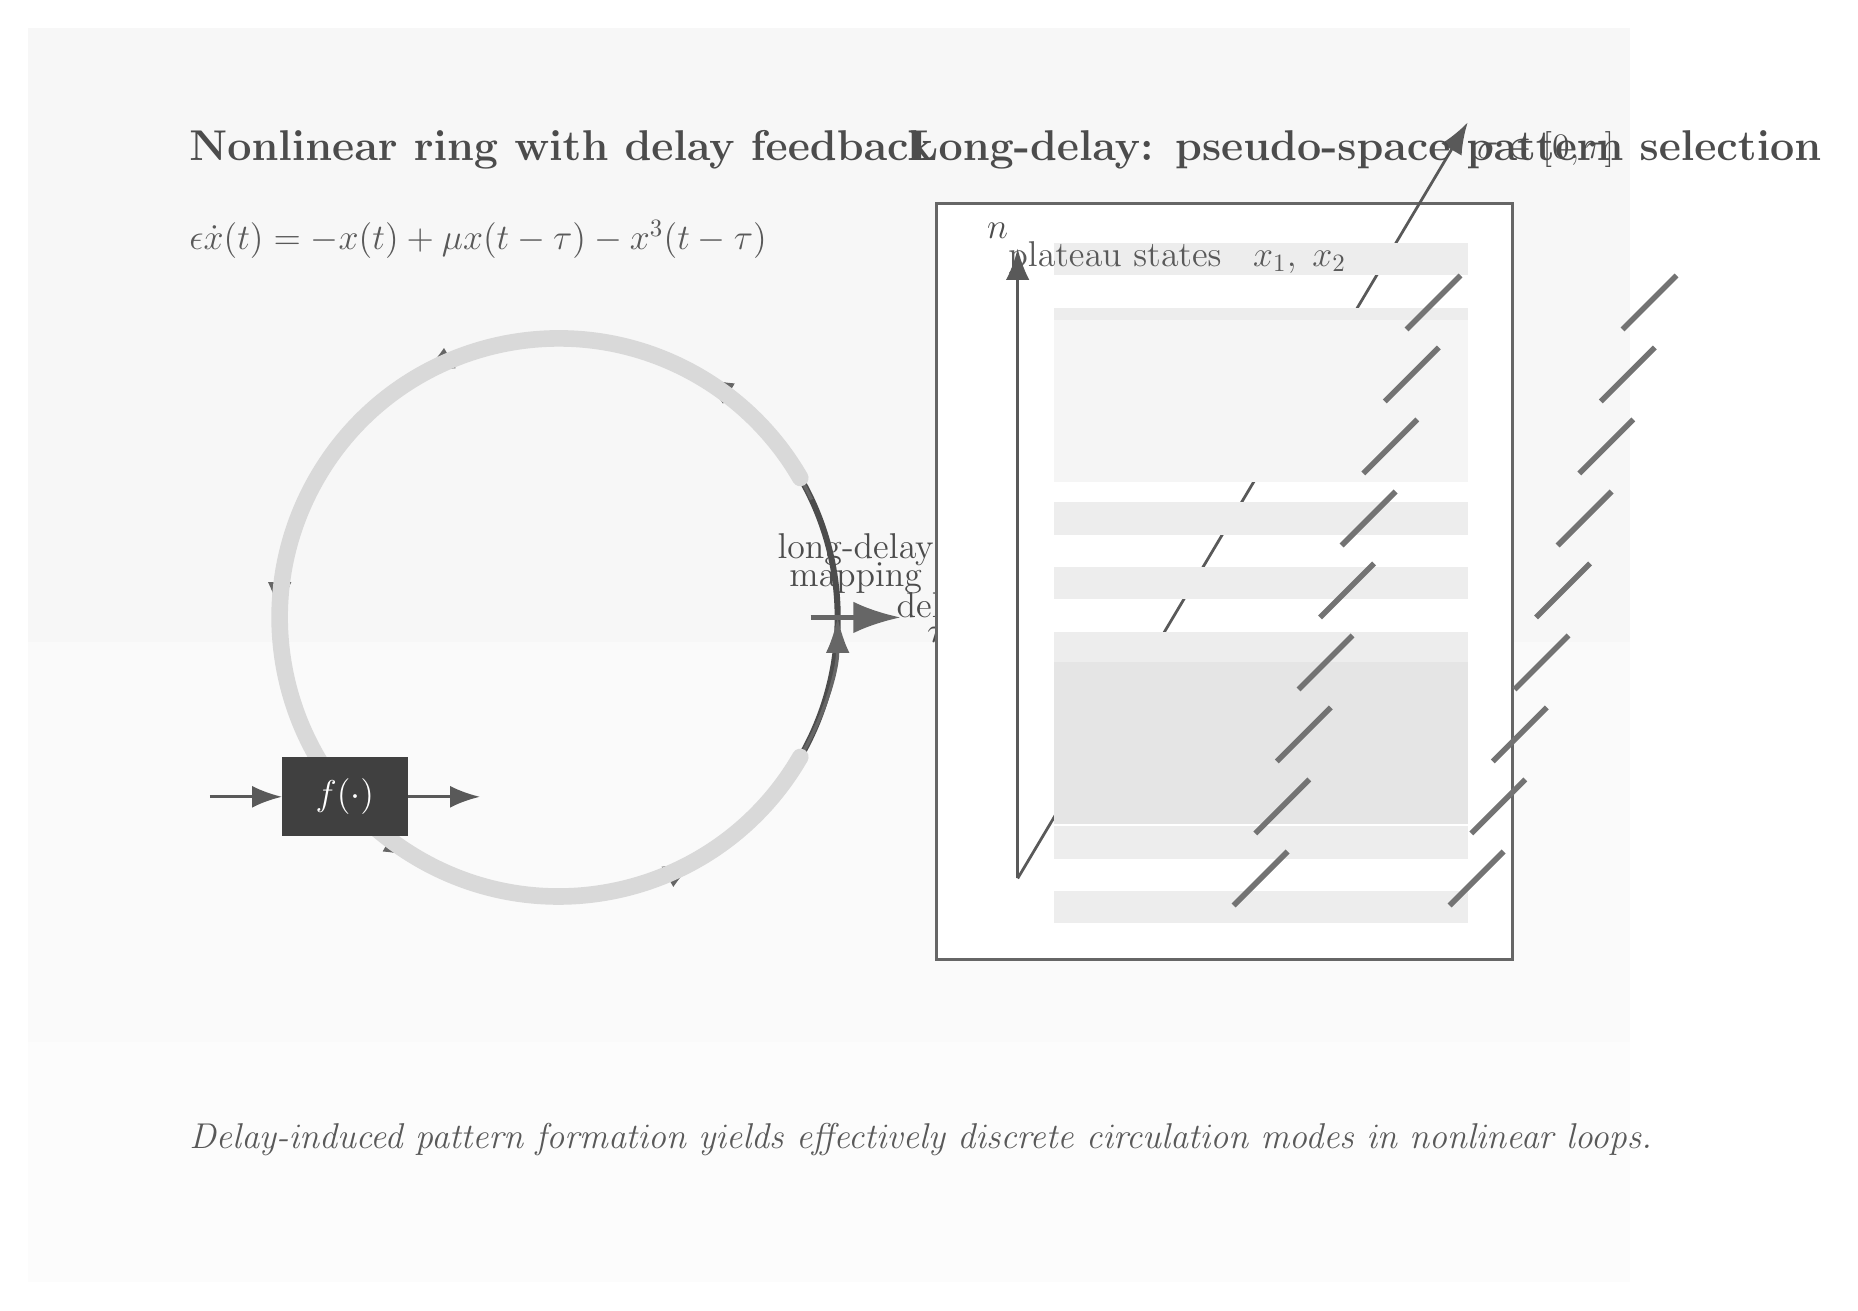
\begin{tikzpicture}[x=1in,y=1in]

        % 1. Canvas Background (Exact dimensions)
        \fill[black!2] (0,0) rectangle (8.0139,6.2739);
        \fill[black!3] (0,3.2) rectangle (8.0139,6.2739);
        \fill[black!1] (0,0) rectangle (8.0139,1.2);

        % 2. Content Scope (Scaled and Shifted)
        \begin{scope}[shift={(0.45, 0.40)}, scale=0.90, transform shape]

            % LEFT PANEL: Ring + delay
            \coordinate (C) at (2.45,3.25);
            \def\R{1.55}

            \draw[line width=2.2pt, black!70] (C) circle (\R);

            \foreach \ang in {25,85,145,205,265,325} {
                \draw[-{Latex[length=4.5mm,width=3.0mm]}, line width=1.2pt, black!60]
                ($(C)+(\ang:\R)$) arc[start angle=\ang, end angle=\ang+35, radius=\R];
            }

            \draw[line width=6pt, black!15, line cap=round]
            ($(C)+(330:\R)$) arc[start angle=330, end angle=30, radius=\R];

            \node[align=center, text=black!70] at ($(C)+(0:\R+0.55)$)
                {\Large delay\\[-2pt]\Large $\tau$};

            \coordinate (NL) at ($(C)+(220:\R)$);
            \fill[black!75] ($(NL)+(-0.35,-0.22)$) rectangle ($(NL)+(0.35,0.22)$);
            \node[text=white] at (NL) {\Large $f(\cdot)$};

            \draw[-{Latex[length=3.8mm,width=2.8mm]}, line width=1.0pt, black!65]
            ($(NL)+(-0.75,0)$) -- ($(NL)+(-0.35,0)$);
            \draw[-{Latex[length=3.8mm,width=2.8mm]}, line width=1.0pt, black!65]
            ($(NL)+(0.35,0)$) -- ($(NL)+(0.75,0)$);

            \node[anchor=west, text=black!70] at (0.35,5.85)
                {\LARGE \textbf{Nonlinear ring with delay feedback}};
            \node[anchor=west, text=black!65] at (0.35,5.35)
                {\Large $\epsilon \dot{x}(t) = -x(t) + \mu x(t-\tau) - x^3(t-\tau)$};

            % RIGHT PANEL: Pseudo-space grid
            \coordinate (PBL) at (4.55,1.35);
            \coordinate (PTR) at (7.75,5.55);

            \fill[white] (PBL) rectangle (PTR);
            \draw[line width=1.2pt, black!60] (PBL) rectangle (PTR);

            \draw[-{Latex[length=4mm,width=3mm]}, line width=1.0pt, black!65]
            ($(PBL)+(0.45,0.45)$) -- ($(PTR)+(-0.25,0.45)$)
            node[below right, text=black!70] {\Large $\sigma \in [0,\tau]$};
            \draw[-{Latex[length=4mm,width=3mm]}, line width=1.0pt, black!65]
            ($(PBL)+(0.45,0.45)$) -- ($(PBL)+(0.45,3.95)$)
            node[above left, text=black!70] {\Large $n$};

            \foreach \k in {0,...,10} {
                \pgfmathsetmacro{\yyA}{1.55 + 0.36*\k}
                \pgfmathsetmacro{\yyB}{\yyA + 0.18}
                \fill[black!7]
                ($(PBL)+(0.65,\yyA-1.35)$)
                rectangle
                ($(PTR)+(-0.25,\yyB-5.55)$);
            }

            \fill[black!10] ($(PBL)+(0.65,0.75)$) rectangle ($(PTR)+(-0.25,-2.55)$);
            \fill[black!4]  ($(PBL)+(0.65,2.65)$) rectangle ($(PTR)+(-0.25,-0.65)$);

            \foreach \m in {0,...,8} {
                \pgfmathsetmacro{\yy}{1.65 + 0.40*\m}
                \pgfmathsetmacro{\shift}{0.12*\m}
                \draw[line width=2.0pt, black!55]
                ($(PBL)+(1.65+\shift,\yy-1.35)$) -- ($(PBL)+(1.95+\shift,\yy-1.05)$);
                \draw[line width=2.0pt, black!55]
                ($(PBL)+(2.85+\shift,\yy-1.35)$) -- ($(PBL)+(3.15+\shift,\yy-1.05)$);
            }

            \node[anchor=west, text=black!65] at ($(PTR)+(-2.85,-0.30)$)
                {\Large plateau states $\;\;x_1,\;x_2$};
            \node[anchor=west, text=black!70] at (4.35,5.85)
                {\LARGE \textbf{Long-delay: pseudo-space pattern selection}};

            % CONNECTOR
            \draw[-{Latex[length=6mm,width=4mm]}, line width=1.6pt, black!60]
            (3.85,3.25) -- (4.35,3.25);

            \node[text=black!70, align=center] at (4.10,3.55)
                {\Large long-delay\\[-2pt]\Large mapping};

            % FOOTER
            \node[anchor=west, text=black!65] at (0.35,0.35)
                {\Large \textit{Delay-induced pattern formation yields effectively discrete circulation modes in nonlinear loops.}};

        \end{scope}
    \end{tikzpicture}
\end{document}